\chapter{Electrostatics}

\textit{We call that fire of the black thunder-cloud 'electricity,' and lecture learnedly about it... but what is it?}\\
\noindent\textbf{-   Thomas Carlyle}

\vspace{1cm}


\begin{marginfigure}%
  \includegraphics[width=\linewidth]{hair_static.jpg}
  \caption{Amber and her charged hair}
  \label{fig:marginfig}
\end{marginfigure}

\marginnote{In the colder months, when the air has less moisture, hair picks up electrical charge.  Fight this unfortunate situation by switching to a more hydrating shampoo and conditioner.}

\section{Background}
Electrostatics deals with the phenomena and properties of stationary charges.   The ancients knew materials such as amber attract lightweight particles after rubbing.   Thales of Miletus made a series of observations on static electricity around 600 BC.  The word electricity comes from the Greek word for amber.  Electrostatic phenomena arise from the forces that electric charges exert on each other.
\begin{itemize}
\item there are two kinds of charge in nature of which opposite attract and like repel
\item charge is conserved
\item charge is quantized
\end{itemize}

\section {Coulomb's Law}

\begin{marginfigure}%
  \includegraphics[width=\linewidth]{torsion.jpg}
  \caption{Coulomb's torsion balance}
  \label{fig:marginfig}
\end{marginfigure}

Coulomb's law describes the electrostatic interaction between electrically charged particles. The law was first published in 1784 by French physicist Charles Augustin de Coulomb. It is analogous to Isaac Newton's inverse-square law of universal gravitation.

$$F_{E}=k_e\frac{q_1q_2}{r^2}$$
$$\overrightarrow{F}_{2\rightarrow 1}=-k_e\frac{q_1q_2}{r^2} \hat{r} \hspace{2cm} \overrightarrow{r}=\overrightarrow{r}_2-\overrightarrow{r}_1$$


$$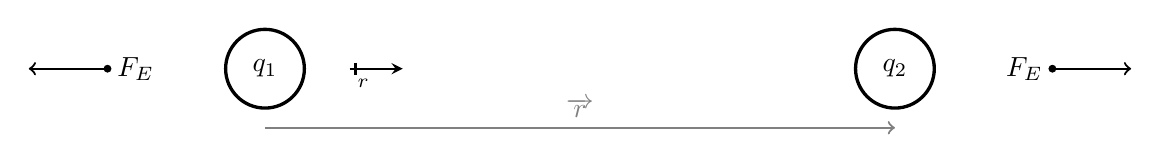
\begin{tikzpicture}[scale=1]
     	
	\fill[black] (-6,0) circle (0.5mm) node [anchor=west ,scale=1] {$F_E$};   
	\draw[->,thick] (-6,0) -- (-7,0) ; 
	\fill[black] (6,0) circle (0.5mm) node [anchor=east,scale=1] {$F_E$};   
	\draw[->,thick] (6,0) -- (7,0) ; 
	 \draw[very thick] (-4,0) circle (0.5cm) node {$q_1$};
	  \draw[very thick] (4,0) circle (0.5cm) node {$q_2$};
	    \draw[thick, color=gray,->] (-4,-0.75) --   (4,-0.75) node [midway, anchor=south] {$\overrightarrow{r}$};
	     
	     
	       \begin{scope}[shift={(-3,0)}, scale=0.75] 
	 
	   \draw[thick](0.2,0.1) -- (0.2,-0.1);
	    \draw[ thick,-stealth] (0.1,0) -- (1,0) node [near start,anchor=north]{\scriptsize $r$};  
	  \end{scope}	     
   \end{tikzpicture}$$


\newpage

\section{Constants}

\begin{table}[h]\index{typefaces!sizes}
  \footnotesize%
  \begin{center}
    \begin{tabular}{lcl}
      \toprule
     Constant & Variable & Quantity \\
      \midrule
 Electrostatic Constant   & $k_e$           & $8.9875 \times 10^{9}\  \nicefrac{ \text{N}\cdot\text{m}^2}{\text{C}^2}$    \\
    Fundamental Charge       & $e$             & $1.6022 \times 10^{-19}\  \text{C}$                                          \\
    Mass of the Electron     & $m_e$           & $9.1095 \times 10^{-31}\  \text{kg}$                                         \\
    Mass of Proton           & $m_p$           & $1.6726 \times 10^{-27} \ \text{kg}$                                         \\ 
    Mass of Neutron           & $m_n$           & $1.6749 \times 10^{-27}\  \text{kg}$                                         \\ 
    Vacuum Permativity       & $\epsilon_0$ & $8.8542 \times 10^{-12}\  \nicefrac{ \text{F}}{\text{m}}$                    \\ 
    Speed of Light       & $c$ & $2.998 \times 10^{8}\  \nicefrac{ \text{m}}{\text{s}}$                    \\ 
      \bottomrule
    \end{tabular}
  \end{center}
  \caption{Physical constants for electrostatics}
  \label{tab:font-sizes}
\end{table}

\marginnote[-50pt]{
$$ k_e=\frac{1}{4\pi \epsilon_0}$$}


\marginnote[0pt]{
The unit of electric charge is the Coulomb, denoted C.}

\section {Electric Field}
The concept of an electric field, or E-field, was introduced by Michael Faraday.  The electric field $\overrightarrow{E}(\overrightarrow{r})$ is a vector field, meaning it is a vector quantity at every point in space.  At a single point in space, the electric field represents the force that would be exerted on a one Coulomb "test charge".  The E-field is the electrostatic force per unit charge.
$$\overrightarrow{E}=\frac{\overrightarrow{F}_e}{q_0}$$
There is an electric field surrounding every charge distribution.  Consider the E-field to represent a feature of space that represents the possibility of electric force, if there were a charge there.
\subsection{Point Charge}
Consider a point charge located at point $\overrightarrow{b}$.  The electric field at a location $\overrightarrow{r}$, due to the presence of the  point charge is represented as follows.  
$$\overrightarrow{E}(\overrightarrow{r})=k_e\frac{q}{R^2}\hat{R} \hspace{1cm} \overrightarrow{R}=\overrightarrow{r}-\overrightarrow{b}$$
A point charge located at the origin of coordinates will generate the following electric field
$$\overrightarrow{E}(\overrightarrow{r})=k_e\frac{q}{r^2} \hat{r} $$

\marginnote[-300pt]{
\subsection{Superposition}
The principle of superposition applied to electrostatic distributions means the force on a given charge $Q$ is the vector sum of forces from interactions with a set of charges.  
$$\overrightarrow{F}_E=k_e\sum_{i=1}^{N} \frac{Qq_i}{R_i^2} \hat{R}_i $$
Equivalently the electric field at a given point in space is the vector sum of the fields due to the set of charges around it.
$$\overrightarrow{E}(\overrightarrow{r})=k_e\sum_{i=1}^{N} \frac{q_i}{R_i^2} \hat{R}_i $$
}


\begin{marginfigure}[-60pt]%
  \includegraphics[width=\linewidth ,trim={7cm 14cm 7cm 7cm},clip]{monopole_graph.pdf}
  \caption{Single positive charge}
  \label{fig:marginfig}
\end{marginfigure}




  \section{Electric Field Lines}
  Electric field lines are a visual tool used to visualize the strength and direction of the electric field in space.  While they are not real, per se, they provide an extremely useful representation for the permeation of electric field through space.  
  \begin{itemize}
 \item Electric field lines emanate perpendicularly out of positive charge and sink perpendicularly into negative charge.  They may also terminate/emanate at infinity if the net charge of the distribution is non-zero.
 \item The number of field lines drawn entering/exiting a charge is proportional to the amount (magnitude) of charge.
 \item  The electric field vector is directed tangent to the field line at each point in space.
 \item No two field lines can cross
 \item  The number of lines per unit area is proportional to the field strength in that area.  Thus $E$ is strong when field lines are close together while $E$ is weak when field lines are far apart.
 \
 \end{itemize}


\begin{marginfigure}[-250pt]%
  \includegraphics[width=\linewidth ,trim={7cm 14cm 7cm 7cm},clip]{dipole_graph.pdf}
  \caption{Dipole field close up}
  \label{fig:marginfig}
\end{marginfigure}

\begin{marginfigure}[-40pt]%
  \includegraphics[width=\linewidth ,trim={7cm 15cm 7cm 8cm},clip]{dipole_far2.pdf}
  \caption{Dipole field far away}
  \label{fig:marginfig}
\end{marginfigure}

\begin{marginfigure}[10pt]%
  \includegraphics[width=\linewidth ,trim={6cm 14cm 6cm 7cm},clip]{Efield_graph2.pdf}
  \caption{Superposition of multiple positive point charges in a row}
  \label{fig:marginfig}
\end{marginfigure}

\begin{marginfigure}[0pt]%
  \includegraphics[width=\linewidth]{electric_fields.jpg}
  \caption{Electric field between two charged plates}
  \label{fig:marginfig}
\end{marginfigure}

%\subsection{Continuous Distribution}
%$$\overrightarrow{E}=k_e\int \frac{dq}{r^2} \hat{r} $$

 
 \section{Charge Distributions}
 A charge distribution is any arrangement of charge in space.  It may consist of a set of various point charges at different locations in space or be a continuous distribution of charge.  Continuous charge distributions may be represented by charge per unit volume, charge per unit area, or charge per unit distance.  These are  types of charge density. 
 $$\text{Volume density} \hspace{2cm} \rho=\frac{Q}{V}$$
  $$\text{Surface density} \hspace{2cm} \sigma=\frac{Q}{A}$$
   $$\text{Line density} \hspace{2cm} \lambda=\frac{Q}{L}$$
   
 \section{Types of Materials}
Atomic lattices making up bulk materials have different electron energy levels or bands.  \textbf{Valence bands} are associated with individual atomic orbital.  Their electrons are spatially localized and lower energy.   \textbf{Conduction bands} are associated with delocalized or free electrons able to move throughout the bulk material.  The energy difference between the highest valence band and lowest conduction band is known as the \textbf{band gap}.  Electrons fill lowest first.  The \textbf{Fermi level} is a thermodynamic property that corresponds to the hypothetical energy of an electron added to the system.  
   
 \newpage  
   
 \begin{description}
  \item[Conductors] In conductors the Fermi level is in conduction band.  This means electrons added to the system are not spatially isolated and is free to move around.  This so called "free charge" accumulates on the surface of the bulk material and congregates more densely in kinks and furrows.
  \item[Insulators]  For insulators the Fermi level in a large band gap.  There are no free electrons.  They are bound locally.  Charge is not free to move around.
   \item[Semiconductors]  In semiconductors the band gap is small so electrons can be easily bumped from localized states to delocalized states in conduction bands.
\end{description}
  
   
   \begin{marginfigure}[-180pt]%
  \includegraphics[width=\linewidth]{conductor.jpg}
  \caption{Electric field and charge distribution in a conducting sphere}
  \label{fig:marginfig}
\end{marginfigure}

\begin{marginfigure}[40pt]%
  \includegraphics[width=\linewidth]{conductor2.jpg}
  \caption{Electric field inside and outside a conducting sphere}
  \label{fig:marginfig}
\end{marginfigure}
   
 \section{Field and Charge Distributions in Conductors}
 \begin{itemize}
 \item The electric field is zero everywhere inside the conductor.
 \item  Any charge on an isolated conductor resides on its surface.
 \item  The electric field just outside a charged conductor is perpendicular to the surface and has a magnitude of $\frac{\sigma}{2\epsilon_0}$.
 \item On an irregularly shaped conductor, charge tends to accumulate at locations where the radius of curvature is smallest such as edges, corners and points.
 \end{itemize}
 

\begin{marginfigure}[80pt]%
  \includegraphics[width=\linewidth]{charge_particle.jpg}
  \caption{Motion of charged particle between two charged plates}
  \label{fig:marginfig}
\end{marginfigure}

 \section{Motion of a Charged Particle}
 Electromagnetic forces are similar to gravity in their relationship to space but are extremely different in one respect.  In gravity mass is responsible for gravitational force but also provides inertia.  For charged particles charge is the source of the electrostatic force but mass still provides the inertia.  
 $$\overrightarrow{F}_{net}=m\overrightarrow{a}$$
 $$\overrightarrow{F}_{net}=q\overrightarrow{E} \hspace{1cm} \longrightarrow \hspace{1cm} \overrightarrow{a}=\frac{q}{m}\overrightarrow{E}$$
 If we generate a field in space and drop a particle in that field then the charge-to-mass ratio can be known through measuring the acceleration.

\newpage

\begin{marginfigure}[50pt]%
  \includegraphics[width=\linewidth]{normal.jpg}
  \caption{Surface normal vector}
  \label{fig:marginfig}
\end{marginfigure}

\begin{marginfigure}[0pt]%
  \includegraphics[width=\linewidth]{gauss_law.jpg}
  \caption{Schematic of Gauss's law }
  \label{fig:marginfig}
\end{marginfigure}

  \section{Electric Flux}
  Electric flux, $\Phi_E$, is the measure electric field passing through a given surface area. Electric flux is proportional to the number of electric field lines perforating the surface.  
  \subsection{Uniform Field Through a Flat Surface}
  For a flat surface and constant field it is the dot product of the electric field vector and the vector normal to the surface.  A surface normal vector points straight out of a surface.
  $$\Phi_E=EA\cos\theta=\overrightarrow{E}\cdot \overrightarrow{A}$$  
  \subsection{Variable Field Through a Set of Flat Surfaces}
  For a variable field through a set of flat surfaces simply take the sum of the flux through all of the surfaces.
  $$\Phi_E=\sum_{i=1}^{N} \overrightarrow{E}_i\cdot \overrightarrow{A}_i$$
   \subsection{Variable Field Through a Continuous Surface}
   A variable field through a continuous smoothly curved surface is modeled as the limit of area elements going to zero. 
   $$\Phi_E=\lim_{\Delta A \rightarrow 0 }\sum_{i=1}^{N} \overrightarrow{E}_i\cdot \Delta \overrightarrow{A}_i$$
   
   \marginnote[-100pt]{
    $$\lim_{\Delta A \rightarrow 0 }\sum_{i=1}^{N} \overrightarrow{E}_i\cdot \Delta \overrightarrow{A}_i=\lim_{\Delta V \rightarrow 0 }\sum_{j=1}^{M} \nabla \cdot \overrightarrow{E}_i\Delta {V}_i$$
}

 \marginnote[-50pt]{
    $$q_{enc}=\lim_{\Delta V \rightarrow 0 }\sum_{j=1}^{M} {\rho}_i\Delta {V}_i$$
}

   \marginnote{
    $$ \nabla \cdot \overrightarrow{E}_i=\frac{ {\rho}_i}{\epsilon_0}$$
}
     \section{Gauss's Law}
     Gauss's law states the total of the electric flux out of a closed surface is equal to the charge enclosed divided by the permittivity.
    \subsection{Variable Field Through a Continuous Closed Surface}
    $$\Phi_E=\lim_{\Delta A \rightarrow 0 }\sum_{i=1}^{N} \overrightarrow{E}_i\cdot \Delta \overrightarrow{A}_i=\frac{q_{inc}}{\epsilon_0}$$
     \subsection{Uniformly Normal Field of Constant Magnitude Through a Continuous Closed Surface}
     $$\Phi_E=EA=\frac{q_{inc}}{\epsilon_0}$$
     
 

 \begin{marginfigure}[-100pt]%
 $$ \includegraphics[width=\linewidth]{gauss_money.jpeg}$$
  \caption{Gauss on money }
  \label{fig:marginfig}
\end{marginfigure}

    \newpage

  \section{Work and Electrostatic Potential Energy}
   
  \marginnote[0pt]{The potential energy $U$ is undetermined up to a constant.  The real physically measurable quantity is the change in potential energy, $\Delta U$.}
  
  \marginnote[10pt]{An individual particle does not have potential energy, $U$ resides in the field (if anywhere) and "belongs" to the system as a whole.  If two charged particles are in proximity they do not each have a potential energy.  There is one electrostatic potential energy between the two particles.}
  
  \marginnote[10pt]{Potential energy is only a meaningful concept for certain types of forces, namely conservative forces.  Remember, the total work done on a particle moving from point $A$ to point $B$ must be independent of path for conservative forces.  }
  
  Electrostatic potential energy, $U$, that results from Coulomb forces and is associated with the configuration of a particular set of point charges within a defined system.  An object contributes to the electrostatic potential energy of a system due to its own electric charge and its relative position to other electrically charged objects.
 
  Recall the definition for change in potential energy and the definition of work.
  $$\Delta U=-W \hspace{1cm} W= \sum_A^B \overrightarrow{F}\cdot \Delta\overrightarrow{s}$$
  Combining the above, and expressing the force in terms of the field, yields the following equation.
  $$\Delta U =- q_0 \sum_A^B \overrightarrow{E}\cdot \Delta\overrightarrow{s}$$
  Consider path-summation on the right hand side of the equation.  Note it is purely a function space, the field in the space and the path.  It is independent of the charge.  In addition, since the electrostatic force is conservative, this path-summation is path-independent.   Therefore it only depends on the endpoints of the path and not the path itself.
  
  \section{Electric Potential}
   \marginnote[0pt]{$$\text{Volt}\equiv\frac{\text{Joule}}{\text{Coulomb}}$$}
    \marginnote[0pt]{ }
  We name the field path-summation $\Delta V$, the change in electric potential.
  $$\Delta V=-\sum_A^B \overrightarrow{E}\cdot \Delta \overrightarrow{s}$$
  $\Delta V$ can be considered the change in electrostatic potential energy per unit charge.
  $$\Delta V=\frac{\Delta U}{q_0}$$
  Finally, after choosing a zero reference, we can write the equation representing the voltage (electric potential) as the electric potential energy per unit charge.
  $$V(\overrightarrow{r})=\frac{U(\overrightarrow{r})}{q_0}$$
   \begin{marginfigure}[0pt]%
 $$ \includegraphics[width=\linewidth]{volt.jpg}$$
  \caption{Alessandro Giuseppe Antonio Anastasio Volta showing his experiments in electricity to Napolean Bonaparte}
  \label{fig:marginfig}
\end{marginfigure}
  The electric potential is a scalar field.  Like the electric field, it is a feature of space independent of the charge we put in the space.  While the electric field represents a vector quantity at every point in space, the voltage (electric potential) represents a single value quantity (scalar quantity) at every point in space.
  
  \newpage
  
  \subsection{Uniform Field}
  \begin{marginfigure}[-10pt]%
  \includegraphics[width=\linewidth ,trim={6cm 14cm 6cm 7cm},clip]{Efield_graph_eq.pdf}
  \caption{Superposition of multiple positive point charges in a row}
  \label{fig:marginfig}
\end{marginfigure}
  Consider the situation of a uniform field, like that between two infinitely large charged plates.
  $$\Delta V=-\sum_A^B \overrightarrow{E}\cdot \Delta \overrightarrow{s}=-E\sum_A^B \Delta S=-E (B-A)=-ED$$
  In this case the potential varies linearly.  This is known as Ed's law.  It is generally applicable at a scale where the field is constant.
  \subsection{Point Charge}
  \begin{marginfigure}[0pt]%
  \includegraphics[width=\linewidth ,trim={7cm 14cm 7cm 7cm},clip]{Efield_graph3.pdf}
  \caption{Single positive charge with equipotential lines}
  \label{fig:marginfig}
\end{marginfigure}
  The potential around a point charge has the familiar $\frac{1}{r}$ dependence.
$$V=k_e\frac{q}{r} $$

\begin{marginfigure}[0pt]%
  \includegraphics[width=\linewidth ,trim={7cm 14cm 7cm 7cm},clip]{dipole_graph_eq.pdf}
  \caption{Dipole field with equipotential lines}
  \label{fig:marginfig}
\end{marginfigure}

\subsection{Superposition of Point Charges}
$$V=k_e\sum_{i=1}^{N} \frac{q_i}{r_i} $$

%\subsection{Continuous Distribution}
%$$V=k_e\int \frac{dq}{r}$$



   \subsection{Vector Field, Scalar Field and Gradient}
     $$\overrightarrow{E}=-\lim_{\Delta \rightarrow 0}\left[\begin{array}{c} \nicefrac{\Delta V}{\Delta x} \\ \nicefrac{\Delta V}{\Delta y} \\ \nicefrac{\Delta V}{\Delta z}\end{array}\right]=-\lim_{\Delta \rightarrow 0}\left[\begin{array}{c} \nicefrac{\Delta }{\Delta x} \\ \nicefrac{\Delta }{\Delta y} \\ \nicefrac{\Delta }{\Delta z}\end{array}\right]V=-\nabla{V}$$
   \subsection{Equipotential Surfaces}
   Equipotential lines, or surfaces in 3-D, are equivalent to contour lines on a topographical map showing lines of equal elevation.
   \begin{itemize}
   \item An equipotential surface is any surface consisting of a continuous distribution of points held at the same electric potential.
   \item Electric field lines intersect equipotential lines at right angles.  They are perpendicular.
   \item Connected conductors share the same potential value.
   \end{itemize} 
